\documentclass[oneside]{book}
\usepackage[utf8]{inputenc}
\usepackage[spanish]{babel}
\usepackage{cite,url,graphicx,epsfig,amsmath,amssymb,enumitem,amsthm,appendix,authblk}
\usepackage[hidelinks,bookmarks=true]{hyperref}
\usepackage[paperwidth=17cm,paperheight=22.5cm,margin=2cm]{geometry} %dimensiones oficiales 

%\setlength{\parskip}{6pt} %espacio entre párrafos

%\usepackage[letter,center,noinfo]{crop} %para revision ("frame" para cuadrito)
%\usepackage{fullpage} %otra pra revision
\newcommand{\thesisTitle}{Flujos de trabajo intensivos en datos para cómputo en la nube}

\usepackage{color} %colores para el codigo
\definecolor{mygreen}{rgb}{0,0.6,0}
\definecolor{mygray}{rgb}{0.5,0.5,0.5}
\definecolor{mymauve}{rgb}{0.58,0,0.82} 

\usepackage{listings}
\usepackage{courier} %para poner codigo en monospace
%\usepackage{iconsolata}
\lstset{ %
  framextopmargin=50pt,
  backgroundcolor=\color{white},      % choose the background color
  basicstyle=\footnotesize\ttfamily,  % size of fonts used for the code
  breaklines=true,                    % automatic line breaking only at whitespace
  captionpos=b,                       % sets the caption-position to bottom
  commentstyle=\color{mygreen},       % comment style
  escapeinside={\%*}{*)},             % if you want to add LaTeX within your code
  keywordstyle=\color{blue},          % keyword style
  stringstyle=\color{mymauve},        % string literal style
  numbers=left,                       % numbering position
  escapeinside={(*@}{@*)}             % labels inside code
}
\renewcommand{\lstlistingname}{Código}
\renewcommand{\lstlistlistingname}{Lista de \lstlistingname s}


\usepackage{algorithm} % Pseudocódigo de algoritmos (Gracias Andreu)
\usepackage{algpseudocode}
\renewcommand{\algorithmicrequire}{\textbf{Entrada:}}
\renewcommand{\algorithmicensure}{\textbf{Salida:}}

\newtheorem{defn}{Definición} %definición de definicones matemágicas

\begin{document}
%%\addtocontents{toc}{Portada}
\begin{titlepage}
\begin{center}

\textsc{\underline{INSTITUTO TECNOLÓGICO AUTÓNOMO DE MÉXICO}}\\[1.5cm] % University name
%\textsc{\Large Tesis}\\[0.5cm] % Thesis type

\begin{figure}[h]
\centering
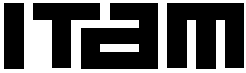
\includegraphics[scale=2]{imagenes/logoitam.png}\\[0.5cm] % Horizontal line
\end{figure} 

\huge{\thesisTitle}\\[1.5cm] % Thesis title


\large \textbf{TESIS}\\ QUE PARA OBTENER EL TÍTULO DE\\ \textbf{MAESTRO EN CIENCIAS EN COMPUTACIÓN}\\[0.8cm]
\large \textbf{P\ \  R\ \  E\ \  S\ \  E\ \  N\ \  T\ \  A}\\[0.8cm]

\textbf{FERNANDO AGUILAR REYES}\\[1.0cm]

\large ASESOR: \textbf{DR. JOSÉ OCTAVIO GUTIÉRREZ GARCÍA}\\[1.4cm]

\large \textbf{MÉXICO, D.F.} {\ \ \ \ \ \ \ \ \ \ \ \ \ \ \ \ \ \ \ \ \ \ \ \ \ \ \ \ \ \ \ \ \ \ } \textbf{2015}

\vfill
\end{center}

\end{titlepage}
 %Portada ITAM 

%\frontmatter
%\thispagestyle{empty}
\noindent Con fundamento en los artículos 21 y 27 de la Ley Federal del Derecho de Autor y como titular de los derechos moral y patrimonial de la obra titulada ``\thesisTitle'', otorgo de manera gratuita y permanente al Instituto Tecnológico Autónomo de México y a la Biblioteca Raúl Bailléres Jr., autorización para que fijen la obra en cualquier medio, incluido el electrónico, y la divulguen entre sus usuarios, profesores, estudiantes o terceras personas, sin que pueda percibir por tal divulgación una contraprestación.\\\\\\\\

\begin{center} 
Fernando Aguilar Reyes\\
\par\noindent\makebox[2.5in]{ }\\
\par\noindent\makebox[2.5in]{\hrulefill}\\
\par\noindent\makebox[2.5in][c]{Fecha}\\
\par\noindent\makebox[2.5in]{ }\\
\par\noindent\makebox[2.5in]{\hrulefill}\\
\par\noindent\makebox[2.5in][c]{Firma}\\
%Fecha:\\
%\rule[1em]{25em}{0.5pt} % This prints a line for the signature 
%Firma:\\
%\rule[1em]{25em}{0.5pt} % This prints a line to write the date
%}
\end{center}
\clearpage % Start a new page
 %Declaracion de derechos
%\begin{center}
Resumen
\end{center}
\noindent En este trabajo se desarroll\'o un algoritmo de planificaci\'on de flujos de trabajo con enfoque a entornos de c\'omputo en la nube, con la capacidad de calcular el número de máquinas necesarias para reducir el tiempo de espera de tareas por recursos disponibles. Tambi\'en, se implement\'o este algoritmo en un software simulador de flujos de trabajo. Los resultados experimentales muestran que el algoritmo reduce los costos de ejecuci\'on de mejor manera que los algoritmos MinMin y Miope. Por \'ultimo, se implement\'o un sistema administrador de flujos de trabajo en la nube, llamado sweeper, con el objetivo de explorar cu\'ales son los retos a los que hay que enfrentarse para llevar este tipo de algoritmos de planifcaci\'on a entornos reales.
\\\\
\noindent \emph{Palabras clave}: Planificación de flujos de trabajo, Programaci\'on din\'amica, Optimizaci\'on de costos

\begin{center}
Abstract
\end{center}
\noindent In this work we developed a workflow scheduling algorithm with a focus on cloud computing environments. This novel algorithm can compute the number of machines required to reduce task waiting time for available resources. Also, this algorithm was implemented in a workflow simulator software. The experimental results show that the algorithm reduces execution costs better than the Myopic algorithm. Finally, a prototype cloud workflow manager system, called sweeper, was developed, with the goal of exploring what are the challenges we need to face in order to use those workflow scheduling algorithms on real life scenarios.
\\\\
\noindent \emph{Keywords}: Workflow scheduling, Dynamic programming, Cost optimizacion

\clearpage
%%\addtocontents{toc}{Agradecmientos}
\begin{center}
{\huge \bfseries Agradecimientos\\}
\end{center}


A Marisela, por apoyarme en todo momento para hacer de la maestr\'ia todo un \'exito.

Al profesor Octavio Gutiérrez, por sus sabios consejos.

A Fernando Esponda y a V\'ictor Gonz\'alez, por otorgarme la opotunidad de estudiar la maestria.

A mi familia, Miguel y Florinda, Rodrigo y Mike.

A Propiedades.com, por facilitar los recursos tecnol\'ogicos para realizar este trabajo.

%\tableofcontents
%\listoffigures
%\lstlistoflistings

%\mainmatter
\chapter{Introducción}

El mundo digital dominado por datos requiere la utilización de algoritmos, tecnologías y mecanismos que permitan orquestar procesamientos de grandes volúmenes de datos, los cuales pueden tardar horas e, incluso, días en completarse. Aún así, el diseño de la aplicación, junto con el flujo de trabajo requiere un esfuerzo considerable cuando se realizan estas aplicaciones.

Ahora bien, sería deseable desarrollar una plataforma que permita distribuir estos flujos de trabajo computacionalmente intensivos en un sistema distribuído con el fin de disminuir el tiempo de ejecución del flujo. También, es deseable disminuir el presupuesto utilizado, ya que es muy común que en los modelos de cómputo en la nube se tenga un modelo económico en que se cobre por utilizar estos servicios.

En este trabajo se muestra el desarrollo de esta plataforma de ejecución de flujos de trabajo intensivo en datos con aplicación en cómputo en la nube. También se muestra el marco teórico necesario para el desarrollo de este proyecto.

Primero, empezaremos por describir el modelo de costos de cómputo en la nube, marcado por acuerdos de nivel de servicio, y se describirá un mecanismo para poder

Luego, describiremos cómo hacer benchmarking dentro de plataformas de cómputo en la nube. Se sugiere utilizar el benchmark proporcionado por LINPACK, ya que éste puede aproximar el rendimiento de un sólo núcleo y varios núcleos. En la tesis de XXX et al. se puede mostrar. Luego describiremos el algoritmo de planificación de flujos de trabajo. Luego describiremos el mecanismo para poner las tareas en de. Luego, compararemos con soluciones existentes como Aneka, HTCondor y Pegasus.


\section{Descripción del problema}

Se tiene un flujo de trabajo definido por $W = (T, D)$, donde $T$ es el conjunto de tareas del flujo de trabajo y $D$ es el conjunto de dependencias que existen entre las tareas del flujo de trabajo. Se desea planificar las tareas en un conjunto de recursos $R$ en la nube de diferente capacidad, los cuales están conectados entre sí por medio de una red privada virtual. Se tiene una función $F: W \times R \mapsto (\mathcal{R}^{+} \times {R}^{+}) $ la cual asocia un costo y un tiempo total de ejecución a una planificación de este flujo de trabajo con el conjunto de recursos dato. Se requiere minimizar la función $F$ tanto en costo como en tiempo. Cabe aclarar que, a diferencia del problema clásico de planificación de flujos de trabajo donde se tiene


\section{Lineamientos de diseño}

Desarrollar un sistema de administración de flujos de trabajo es como desarrollar una receta para hacer chocolate: hay muchas formas y modalidades de hacerlo. Sin embargo, se pueden ver algunos patrones de uso o generalidades que quisiéramos observar en el sistema administrador de flujos de trabajo. A continuación, se listarán los lineamentos de diseño deseables en el sistema administrador de flujos de trabajo.



\subsection{El flujo como centro de la aplicación}

Los sistemas de cómputo distribuido tienen inherentes una complexidad que crece más conforme mayores capacidades de agregan a éstos. Los científicos y personas especialistas de algún dominio de conocimiento cada vez tienen menos tiempo para aprender los detalles del funcionamiento de estos sistemas distribuidos. Por otro lado, dibujar diagramas que describan la secuencia de ejecución de los programas es más intuitivo. Y un flujo de trabajo bien puede expresarse a través de estos diagramas. De esta forma, especificar el flujo de trabajo es el pilar que describe los procesos a ejecutar. Por otro lado, el flujo de trabajo aporta información que ayuda a la paralelización y ejecución distribuida del mismo.



\subsection{Orientado a nubes}

Aunque se pueden ejecutar Open Grid Scheduler, HTCondor, programas MPI y aplicaciones basadas en MapReduce y cómputo distribuido en gráficas, éstos funcionan muy bien en entornos de una sola computadora con gran capacidad o en grids institucionales. Sin embargo, cuando se utilizan estos programas en enfoques como la nube, surgen algunas eventualidades, a saber: 1) es más difícil supervisar estos entornos por el hecho de la insfraestrucutra no es \emph{on-premise} o, en el caso de grids comunitarios, se conoce a ciencia cierta el funcionamiento del sistema y, 2) hay un costo monetario por utilizar estos recursos que está explícitamente establecido, el cual es deseable minimizar. Además, otra característica importante de la nube, a saber, la utilización de máquinas virutales, hace que el rendimiento del sistema distribuido en general pueda escalarse prácticamente sin límites. Por ello, es deseable ejecutar el flujo de trabajo en el menor tiempo posible, respetando un presupuesto asignado. Esta flexibilidad sólo es posible encontrarla actualmente en las infraestructuras de servicios de cómputo en la nube. Por esta razón, el sistema administrador de flujos de trabajo tiene que estar fuertemente orientado a trabajar en la nube.



\subsection{Intensivo en datos}

Como se ha dicho en la introducción, las cargas de trabajo que administran estos sistemas usualmente generan enormes cantidades de datos, que son desde logs de operación, archivos intermedios de resultados o volcados de memoria en caso de que ocurra algún error. Así, manejar datos es primordial en nuestra solucíón. Este requerimiento se puede cumplir utilizando sistemas de archivos distribuidos con énfasis en la tasa de rendimiento de datos guardados.


\subsection{Portable entre nubes}

Esto con el fin de tener la libertad de escoger la plataforma de cómputo en la nube conveniente a las necesidades del flujo.
%Aunque dudo que este requerimiento pueda cumplirse, debido a las abstracciones necesarias que deben hacerse en el software


\subsection{Simple}

Las interacciones con el usuario deben ser simples



\subsection{Basado en estándares}

%\include{chap02-workflows}
%\include{chap03-distributed_computing}
%\include{chap04-scheduling}
%\include{chap05-scheduling_algorithms}
%\include{chap06-workflow_mgmt_software}
%\include{chap07-implementation}
%\include{chap08-results}
%\include{chap09-conclusions}

%\appendix
%\chapter{Resultados de ejecución}

\section{Tiempos totales de ejecución}


% latex table generated in R 3.3.1 by xtable 1.8-2 package
% Tue Nov  1 23:39:33 2016
\begin{longtable}{rrrrrrr}
  \hline
N & Nodos & Aristas & Ciego & MaxMin & MinMin & Miope \\ 
  \hline
  0 &  33 &  48 & 13.09 & 3.70 & 3.56 & 5.71 \\ 
    1 &  13 &  22 & 6.06 & 4.15 & 4.41 & 4.70 \\ 
    2 &  44 &  96 & 9.83 & 3.64 & 3.86 & 5.64 \\ 
    3 &  31 &  38 & 6.73 & 2.22 & 2.14 & 2.81 \\ 
    4 &  49 &  95 & 13.83 & 2.05 & 2.11 & 4.48 \\ 
    5 &  33 &  63 & 10.78 & 4.35 & 4.52 & 7.71 \\ 
    6 &  32 &  47 & 8.37 & 2.47 & 2.70 & 3.25 \\ 
    7 &  12 &  18 & 6.78 & 4.43 & 4.22 & 5.12 \\ 
    8 &  31 &  52 & 10.74 & 3.11 & 2.99 & 4.63 \\ 
    9 &  50 &  97 & 19.22 & 5.12 & 5.06 & 8.56 \\ 
   10 &  50 &  72 & 7.87 & 1.32 & 1.33 & 2.43 \\ 
   11 &  36 &  76 & 9.93 & 3.35 & 3.67 & 6.34 \\ 
   12 &  47 & 104 & 16.72 & 2.94 & 3.12 & 6.98 \\ 
   13 &  28 &  30 & 6.92 & 1.15 & 1.19 & 2.76 \\ 
   14 &  39 &  62 & 10.74 & 3.25 & 3.38 & 4.28 \\ 
   15 &  26 &  33 & 5.26 & 1.72 & 1.70 & 2.88 \\ 
   16 &   8 &  11 & 4.27 & 2.58 & 2.88 & 3.84 \\ 
   17 &   4 &   3 & 2.16 & 1.23 & 1.57 & 1.63 \\ 
   18 &   6 &   5 & 2.71 & 2.08 & 1.72 & 1.87 \\ 
   19 &  18 &  19 & 4.61 & 1.59 & 1.66 & 2.32 \\ 
   20 &  24 &  32 & 7.94 & 2.29 & 2.35 & 4.01 \\ 
   21 &  14 &  23 & 5.78 & 3.10 & 3.51 & 3.73 \\ 
   22 &  35 &  96 & 14.96 & 4.93 & 5.35 & 9.08 \\ 
   23 &  15 &  18 & 4.60 & 2.86 & 3.40 & 3.98 \\ 
   24 &   2 &   1 & 1.41 & 1.41 & 1.41 & 1.41 \\ 
   25 &  42 &  78 & 10.50 & 3.90 & 3.75 & 4.36 \\ 
   26 &  24 &  53 & 11.14 & 6.16 & 6.00 & 7.84 \\ 
   27 &  28 &  45 & 9.81 & 2.73 & 2.89 & 4.19 \\ 
   28 &  42 &  94 & 13.19 & 4.21 & 4.74 & 5.85 \\ 
   29 &  42 &  78 & 12.59 & 1.88 & 2.01 & 4.73 \\ 
   30 &   4 &   3 & 2.71 & 2.71 & 2.71 & 2.71 \\ 
   31 &   1 &   0 & 0.76 & 0.76 & 0.76 & 0.76 \\ 
   32 &   3 &   2 & 2.28 & 2.28 & 2.28 & 2.28 \\ 
   33 &  26 &  42 & 7.42 & 1.47 & 1.48 & 2.92 \\ 
   34 &  47 &  61 & 6.24 & 1.17 & 1.12 & 2.44 \\ 
   35 &  30 &  41 & 8.49 & 2.99 & 2.98 & 5.44 \\ 
   36 &  24 &  25 & 5.06 & 2.19 & 2.17 & 2.76 \\ 
   37 &  22 &  52 & 7.38 & 2.66 & 3.01 & 4.54 \\ 
   38 &  28 &  38 & 7.63 & 1.27 & 1.28 & 2.71 \\ 
   39 &  42 &  81 & 11.96 & 3.97 & 4.39 & 6.30 \\ 
   40 &  17 &  23 & 4.26 & 1.52 & 1.52 & 2.66 \\ 
   41 &  48 &  76 & 7.21 & 2.47 & 2.58 & 4.13 \\ 
   42 &  37 &  58 & 11.43 & 4.77 & 5.18 & 6.75 \\ 
   43 &  15 &  16 & 2.66 & 0.94 & 0.93 & 1.39 \\ 
   44 &  27 &  57 & 11.58 & 3.92 & 4.30 & 7.16 \\ 
   45 &  21 &  37 & 7.76 & 4.61 & 4.65 & 5.57 \\ 
   46 &  10 &  13 & 2.95 & 1.38 & 1.30 & 2.30 \\ 
   47 &  20 &  23 & 4.34 & 0.84 & 0.87 & 1.42 \\ 
   48 &  24 &  34 & 7.79 & 3.08 & 3.09 & 3.70 \\ 
   49 &   6 &   6 & 2.65 & 1.95 & 2.12 & 2.72 \\ 
   50 &   5 &   4 & 2.39 & 1.92 & 2.07 & 1.64 \\ 
   51 &  22 &  31 & 4.12 & 1.50 & 1.50 & 2.19 \\ 
   52 &  49 &  85 & 14.19 & 4.13 & 4.17 & 6.12 \\ 
   53 &  32 &  52 & 9.57 & 2.82 & 2.88 & 5.37 \\ 
   54 &  44 &  62 & 8.44 & 1.41 & 1.62 & 2.48 \\ 
   55 &  25 &  45 & 10.72 & 5.86 & 5.90 & 8.10 \\ 
   56 &  23 &  29 & 3.73 & 1.45 & 1.60 & 2.30 \\ 
   57 &   5 &   4 & 1.87 & 1.26 & 1.84 & 1.26 \\ 
   58 &  17 &  22 & 4.80 & 1.69 & 1.83 & 2.31 \\ 
   59 &   6 &   7 & 4.10 & 2.31 & 2.43 & 2.44 \\ 
   60 &  11 &  13 & 4.83 & 3.21 & 3.44 & 3.98 \\ 
   61 &  13 &  17 & 5.68 & 3.35 & 3.95 & 4.68 \\ 
   62 &  46 &  79 & 11.12 & 3.37 & 3.57 & 4.17 \\ 
   63 &  40 &  64 & 15.22 & 4.19 & 4.36 & 6.80 \\ 
   64 &  16 &  20 & 3.99 & 1.60 & 1.49 & 2.44 \\ 
   65 &  20 &  35 & 7.82 & 2.42 & 2.29 & 3.96 \\ 
   66 &   3 &   2 & 1.19 & 0.85 & 1.06 & 1.19 \\ 
   67 &  39 &  63 & 5.73 & 2.06 & 2.21 & 2.84 \\ 
   68 &   7 &   7 & 2.95 & 2.39 & 2.44 & 2.17 \\ 
   69 &   1 &   0 & 0.90 & 0.90 & 0.90 & 0.90 \\ 
   70 &  10 &  11 & 5.70 & 3.32 & 3.82 & 4.52 \\ 
   71 &  44 &  71 & 10.04 & 4.04 & 3.93 & 4.33 \\ 
   72 &  15 &  17 & 5.19 & 2.30 & 2.09 & 2.93 \\ 
   73 &  49 &  92 & 13.32 & 4.61 & 4.56 & 5.75 \\ 
   74 &  36 &  67 & 11.09 & 3.39 & 3.38 & 5.02 \\ 
   75 &  36 &  62 & 11.09 & 1.70 & 1.67 & 4.05 \\ 
   76 &  18 &  29 & 6.53 & 2.28 & 2.52 & 3.75 \\ 
   77 &   9 &  11 & 5.15 & 3.33 & 3.08 & 4.00 \\ 
   78 &  35 &  83 & 11.35 & 4.60 & 4.57 & 7.07 \\ 
   79 &  26 &  52 & 6.03 & 1.94 & 2.03 & 3.61 \\ 
   80 &  26 &  44 & 5.71 & 3.04 & 3.17 & 3.97 \\ 
   81 &  48 &  89 & 11.58 & 3.37 & 3.34 & 6.34 \\ 
   82 &  10 &  10 & 2.24 & 0.98 & 0.93 & 1.48 \\ 
   83 &  25 &  29 & 7.02 & 2.56 & 2.60 & 3.75 \\ 
   84 &  40 &  67 & 14.20 & 2.12 & 2.20 & 5.00 \\ 
   85 &  17 &  25 & 5.81 & 2.14 & 2.47 & 3.56 \\ 
   86 &  17 &  20 & 2.94 & 1.31 & 1.35 & 1.76 \\ 
   87 &   8 &   8 & 2.97 & 1.93 & 1.86 & 2.16 \\ 
   88 &  17 &  23 & 4.15 & 1.60 & 1.66 & 2.84 \\ 
   89 &  40 &  69 & 7.86 & 2.67 & 2.62 & 4.44 \\ 
   90 &  45 &  74 & 9.21 & 2.95 & 3.03 & 4.58 \\ 
   91 &  25 &  28 & 4.29 & 1.40 & 1.40 & 1.65 \\ 
   92 &  48 &  79 & 14.87 & 2.77 & 3.10 & 6.44 \\ 
   93 &   9 &  15 & 3.54 & 3.15 & 3.34 & 2.93 \\ 
   94 &   7 &   7 & 4.99 & 2.78 & 2.84 & 3.30 \\ 
   95 &   6 &   5 & 2.02 & 2.06 & 1.81 & 1.82 \\ 
   96 &  17 &  23 & 4.88 & 2.24 & 2.24 & 3.68 \\ 
   97 &   6 &   7 & 3.61 & 1.93 & 2.29 & 2.33 \\ 
   98 &   4 &   3 & 2.54 & 1.56 & 1.71 & 2.06 \\ 
   99 &  44 &  81 & 14.15 & 4.19 & 4.22 & 7.42 \\ 
   \hline
\caption{Tiempos totales de planificación estimado por cada algoritmo de planificación.}
\label{table:makespans}
\end{longtable}


\section{Costos de ejecución}

% latex table generated in R 3.3.1 by xtable 1.8-2 package
% Tue Nov  1 23:57:33 2016
\begin{longtable}{rrrrrrr}
  \hline
N & Nodos & Aristas & Ciego & MaxMin & MinMin & Miope \\ 
  \hline
  0 &  33 &  48 & 222.08 & 107.73 & 89.30 & 203.54 \\ 
    1 &  13 &  22 & 41.28 & 28.12 & 29.46 & 31.76 \\ 
    2 &  44 &  96 & 182.59 & 92.85 & 100.95 & 156.22 \\ 
    3 &  31 &  38 & 136.01 & 73.86 & 65.94 & 109.03 \\ 
    4 &  49 &  95 & 194.67 & 117.40 & 111.45 & 402.13 \\ 
    5 &  33 &  63 & 199.90 & 77.74 & 79.12 & 143.12 \\ 
    6 &  32 &  47 & 80.86 & 75.29 & 79.08 & 131.33 \\ 
    7 &  12 &  18 & 45.49 & 29.28 & 23.64 & 34.07 \\ 
    8 &  31 &  52 & 94.04 & 75.18 & 76.41 & 162.05 \\ 
    9 &  50 &  97 & 193.71 & 167.18 & 164.07 & 382.43 \\ 
   10 &  50 &  72 & 209.41 & 120.61 & 116.80 & 240.85 \\ 
   11 &  36 &  76 & 195.21 & 89.65 & 86.34 & 173.66 \\ 
   12 &  47 & 104 & 236.99 & 134.56 & 117.31 & 426.98 \\ 
   13 &  28 &  30 & 54.52 & 49.36 & 48.94 & 156.84 \\ 
   14 &  39 &  62 & 155.98 & 88.90 & 80.18 & 154.13 \\ 
   15 &  26 &  33 & 61.58 & 52.19 & 45.98 & 119.76 \\ 
   16 &   8 &  11 & 16.95 & 14.17 & 13.24 & 25.89 \\ 
   17 &   4 &   3 & 10.95 & 8.17 & 7.24 & 10.95 \\ 
   18 &   6 &   5 & 14.58 & 13.74 & 11.49 & 10.76 \\ 
   19 &  18 &  19 & 52.12 & 36.94 & 32.36 & 63.62 \\ 
   20 &  24 &  32 & 71.83 & 57.41 & 57.16 & 125.46 \\ 
   21 &  14 &  23 & 29.94 & 25.98 & 24.96 & 35.74 \\ 
   22 &  35 &  96 & 267.08 & 86.49 & 90.73 & 171.75 \\ 
   23 &  15 &  18 & 34.04 & 26.76 & 26.26 & 40.21 \\ 
   24 &   2 &   1 & 3.24 & 3.24 & 3.24 & 3.24 \\ 
   25 &  42 &  78 & 220.44 & 100.68 & 95.30 & 121.93 \\ 
   26 &  24 &  53 & 96.73 & 61.65 & 51.16 & 82.94 \\ 
   27 &  28 &  45 & 106.60 & 73.76 & 75.76 & 139.12 \\ 
   28 &  42 &  94 & 340.49 & 111.60 & 121.20 & 169.83 \\ 
   29 &  42 &  78 & 136.32 & 91.43 & 83.66 & 377.24 \\ 
   30 &   4 &   3 & 6.22 & 6.22 & 6.22 & 6.22 \\ 
   31 &   1 &   0 & 1.74 & 1.74 & 1.74 & 1.74 \\ 
   32 &   3 &   2 & 5.25 & 5.25 & 5.25 & 5.25 \\ 
   33 &  26 &  42 & 59.87 & 55.47 & 45.57 & 167.58 \\ 
   34 &  47 &  61 & 109.45 & 99.79 & 103.18 & 251.95 \\ 
   35 &  30 &  41 & 78.83 & 62.94 & 62.02 & 146.22 \\ 
   36 &  24 &  25 & 69.23 & 55.95 & 45.24 & 74.97 \\ 
   37 &  22 &  52 & 146.86 & 48.62 & 54.50 & 85.06 \\ 
   38 &  28 &  38 & 73.08 & 64.31 & 58.48 & 135.28 \\ 
   39 &  42 &  81 & 150.40 & 92.39 & 80.91 & 167.20 \\ 
   40 &  17 &  23 & 43.33 & 34.50 & 34.40 & 72.60 \\ 
   41 &  48 &  76 & 156.63 & 103.04 & 92.15 & 163.37 \\ 
   42 &  37 &  58 & 120.32 & 85.36 & 91.56 & 129.81 \\ 
   43 &  15 &  16 & 46.56 & 28.49 & 27.08 & 33.76 \\ 
   44 &  27 &  57 & 133.50 & 70.44 & 69.27 & 133.98 \\ 
   45 &  21 &  37 & 69.15 & 48.77 & 42.58 & 57.57 \\ 
   46 &  10 &  13 & 32.83 & 22.93 & 23.50 & 37.68 \\ 
   47 &  20 &  23 & 56.86 & 42.30 & 38.29 & 92.06 \\ 
   48 &  24 &  34 & 86.35 & 54.53 & 54.37 & 72.70 \\ 
   49 &   6 &   6 & 17.71 & 12.85 & 9.73 & 16.40 \\ 
   50 &   5 &   4 & 14.92 & 11.68 & 9.53 & 9.74 \\ 
   51 &  22 &  31 & 46.18 & 42.67 & 41.44 & 64.84 \\ 
   52 &  49 &  85 & 310.20 & 147.36 & 135.11 & 243.31 \\ 
   53 &  32 &  52 & 175.38 & 101.20 & 80.82 & 189.08 \\ 
   54 &  44 &  62 & 173.04 & 99.98 & 87.06 & 205.23 \\ 
   55 &  25 &  45 & 72.59 & 54.92 & 54.05 & 90.15 \\ 
   56 &  23 &  29 & 74.12 & 49.83 & 54.34 & 84.72 \\ 
   57 &   5 &   4 & 8.44 & 8.44 & 8.44 & 8.44 \\ 
   58 &  17 &  22 & 43.85 & 38.86 & 32.81 & 60.69 \\ 
   59 &   6 &   7 & 11.16 & 11.80 & 11.16 & 15.69 \\ 
   60 &  11 &  13 & 22.10 & 20.40 & 21.05 & 26.62 \\ 
   61 &  13 &  17 & 63.91 & 37.14 & 34.75 & 52.40 \\ 
   62 &  46 &  79 & 201.23 & 107.03 & 98.60 & 153.92 \\ 
   63 &  40 &  64 & 103.32 & 103.52 & 103.98 & 235.02 \\ 
   64 &  16 &  20 & 46.23 & 38.50 & 33.96 & 59.67 \\ 
   65 &  20 &  35 & 48.95 & 43.61 & 39.46 & 106.08 \\ 
   66 &   3 &   2 & 8.03 & 5.66 & 4.87 & 8.03 \\ 
   67 &  39 &  63 & 110.00 & 75.82 & 78.33 & 126.35 \\ 
   68 &   7 &   7 & 16.36 & 15.36 & 15.71 & 12.99 \\ 
   69 &   1 &   0 & 2.06 & 2.06 & 2.06 & 2.06 \\ 
   70 &  10 &  11 & 30.35 & 21.89 & 21.47 & 28.37 \\ 
   71 &  44 &  71 & 202.38 & 100.48 & 84.79 & 112.55 \\ 
   72 &  15 &  17 & 40.25 & 34.03 & 33.49 & 47.78 \\ 
   73 &  49 &  92 & 152.04 & 116.19 & 102.95 & 166.80 \\ 
   74 &  36 &  67 & 177.57 & 94.41 & 86.38 & 166.23 \\ 
   75 &  36 &  62 & 140.73 & 103.89 & 103.84 & 396.70 \\ 
   76 &  18 &  29 & 74.23 & 35.21 & 40.58 & 70.99 \\ 
   77 &   9 &  11 & 17.57 & 18.75 & 16.59 & 26.67 \\ 
   78 &  35 &  83 & 152.49 & 74.75 & 74.74 & 127.35 \\ 
   79 &  26 &  52 & 65.48 & 48.11 & 47.23 & 110.34 \\ 
   80 &  26 &  44 & 85.60 & 52.41 & 52.48 & 80.43 \\ 
   81 &  48 &  89 & 169.24 & 111.34 & 117.67 & 289.44 \\ 
   82 &  10 &  10 & 18.59 & 15.09 & 14.97 & 26.17 \\ 
   83 &  25 &  29 & 80.35 & 58.72 & 56.02 & 103.90 \\ 
   84 &  40 &  67 & 158.30 & 102.74 & 87.93 & 353.54 \\ 
   85 &  17 &  25 & 78.67 & 37.25 & 42.67 & 63.26 \\ 
   86 &  17 &  20 & 32.03 & 32.55 & 29.90 & 44.78 \\ 
   87 &   8 &   8 & 13.41 & 14.57 & 13.41 & 20.46 \\ 
   88 &  17 &  23 & 34.68 & 34.30 & 32.53 & 48.24 \\ 
   89 &  40 &  69 & 244.55 & 115.28 & 96.31 & 196.25 \\ 
   90 &  45 &  74 & 179.87 & 102.89 & 102.97 & 203.96 \\ 
   91 &  25 &  28 & 56.84 & 50.99 & 50.94 & 68.13 \\ 
   92 &  48 &  79 & 436.54 & 149.46 & 145.51 & 376.05 \\ 
   93 &   9 &  15 & 18.08 & 19.00 & 19.33 & 19.32 \\ 
   94 &   7 &   7 & 29.47 & 18.17 & 13.04 & 22.70 \\ 
   95 &   6 &   5 & 10.79 & 12.95 & 11.18 & 11.89 \\ 
   96 &  17 &  23 & 48.04 & 37.53 & 32.95 & 63.81 \\ 
   97 &   6 &   7 & 20.04 & 12.89 & 10.51 & 15.63 \\ 
   98 &   4 &   3 & 7.87 & 8.49 & 7.87 & 9.59 \\ 
   99 &  44 &  81 & 257.64 & 132.04 & 117.59 & 280.95 \\ 
   \hline
\caption{Costos de ejecución estimados por cada algoritmo de planificación.}
\label{table:costs}
\end{longtable}


%\bibliographystyle{plain}
%\bibliography{referencias}
\end{document}
